\documentclass[tikz,border=5pt]{standalone}
\usepackage{tikz}
\usetikzlibrary{calc}

\begin{document}
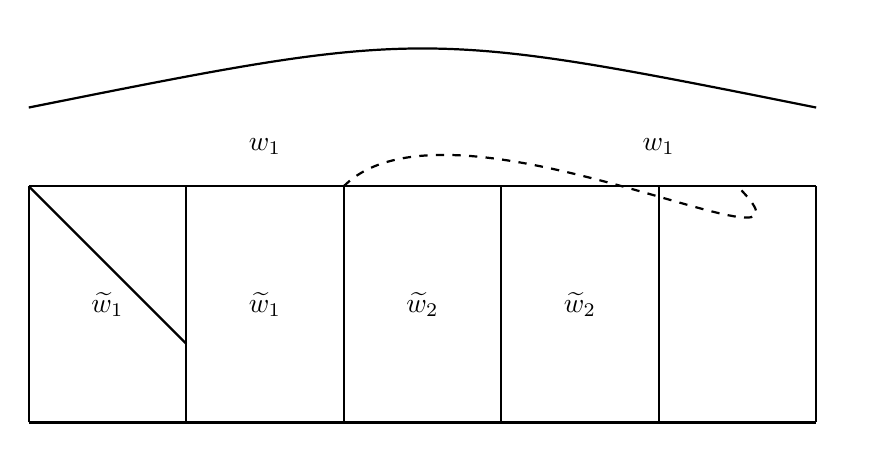
\begin{tikzpicture}[thick]

% Draw vertical lines
\foreach \x in {0, 2, 4, 6, 8, 10} {
    \draw (\x,0) -- (\x,3);
}

% Draw horizontal lines
\draw (0,0) -- (10,0);
\draw (0,3) -- (10,3);

% Draw curved line above the bars
\draw (0,4) .. controls (5,5) .. (10,4);

% Draw w_tilde labels
\node at (1,1.5) {$\widetilde{w}_1$};
\node at (3,1.5) {$\widetilde{w}_1$};
\node at (5,1.5) {$\widetilde{w}_2$};
\node at (7,1.5) {$\widetilde{w}_2$};

% Draw w_1 labels
\node at (3,3.5) {$w_1$};
\node at (8,3.5) {$w_1$};

% Draw dashed line
\draw[dashed] (4,3) to[out=45,in=-45] (9,3);

% Draw diagonal line from top left to bottom right
\draw (0,3) -- (2,1);

\end{tikzpicture}
\end{document}